%************************************************
\chapter{Platform Specific Functionality}\label{ch:ui}
%************************************************

Thanks to the framework we chose to use, and the desire to present our application as natively as possible, there exists the need for some platform specific functionality. Most of this functionality has to do with the \ac{UI} and some third-party libraries.

This chapter will be divided in two parts, one for iOS and one for Android. In here we will also discuss all about the \texttt{callback} functions we mentioned earlier. 

\section{Android UI}

The main reason we chose \textit{Xamarin} as the framework for the development of our application is the fact that we can develop the \ac{UI} in a completely independent fashion.

On the Android side of things, this means using specially crafted \ac{XML} files for defining the look of the application. Under Xamarin Studio, we have two options for laying out the content of each view:  We can use the Android Layout Editor to drag and drop elements form a toolbox or we can  directly edit the \ac{XML} source code and change everything manually.

Since most of the application is composed of Lists and Grids, it is actually easier to manually edit the \ac{XML} source code, than to mess around with the visual editor.

\autoref{list:and_xml} and \autoref{fig:and_layout} show both sides of the same file, the source and how it looks inside the Android Layout Editor.

Decribing what each element inside the \ac{XML} file is, how they work and why they work that way is outside the scope of this work. If you need more information about the inner workings of the Android Operating System, please refer to more specific literature.


\lstset{language=XML}
\begin{lstlisting}[frame=lt,caption=Company.axml, label={list:and_xml}]
<?xml version="1.0" encoding="utf-8"?>
<LinearLayout xmlns:android="http://schemas.android.com/apk/res/android"
    android:orientation="vertical"
    android:layout_width="wrap_content"
    android:layout_height="wrap_content">
    <ImageView
        android:src="@android:drawable/ic_menu_gallery"
        android:layout_width="match_parent"
        android:layout_height="match_parent"
        android:padding="5dip"
        android:gravity="center"
        android:id="@+id/company_image" />
    <TextView
        android:id="@+id/Name"
        android:layout_width="match_parent"
        android:layout_height="wrap_content"
        android:ellipsize="end"
        android:singleLine="true"
        android:textAppearance="?android:attr/textAppearanceSmall"
        android:padding="5dip"
        android:gravity="center"
        android:text="Test" />
</LinearLayout>
\end{lstlisting}


\begin{figure}[H]
    \begin{center}
        {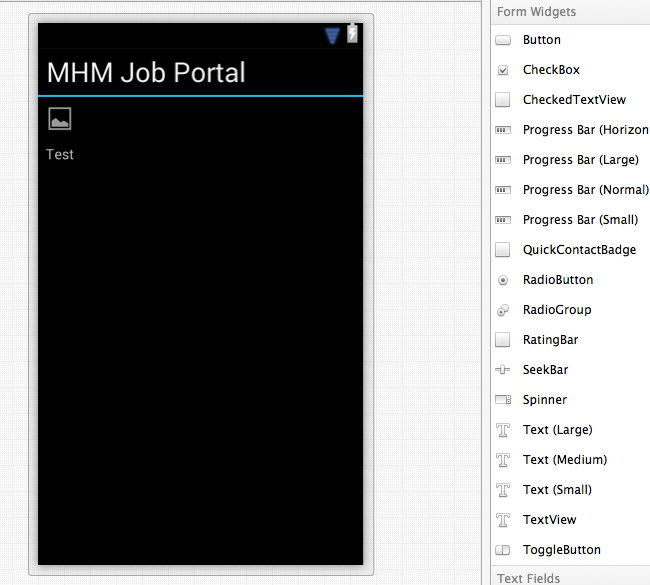
\includegraphics[width=0.75\linewidth]{gfx/and_view}}
        \caption[Android Layout Editor]{Android Layout Editor}\label{fig:and_layout}
    \end{center}
\end{figure}

\subsection{Views, Items and Adapters}
Our Job Portal Aggregator consists of information that is easily packable inside a list, this is why the main view of the application consists of a list of the latest vacancies available.

In order to display this information we need to define a view group where the information will be placed and a view item that represents each element inside the list. All these is done inside the \ac{XML} layout files.

\begin{lstlisting}[frame=lt,caption=Publication.axml, label={list:pub_xml}]
<?xml version="1.0" encoding="utf-8"?>
<LinearLayout xmlns:android="http://schemas.android.com/apk/res/android"
    android:orientation="horizontal"
    android:layout_width="fill_parent"
    android:layout_height="fill_parent">
    <ImageView
        android:src="@android:drawable/ic_menu_gallery"
        android:layout_width="57.2dp"
        android:layout_height="63.0dp"
        android:id="@+id/company_image" />
    <LinearLayout
        android:orientation="vertical"
        android:layout_width="fill_parent"
        android:layout_height="fill_parent">
        <TextView
            android:id="@+id/Title"
            android:layout_width="match_parent"
            android:layout_height="wrap_content"
            android:ellipsize="end"
            android:singleLine="true"
            android:textAppearance="?android:attr/textAppearanceMedium"
            android:padding="5dip"
            android:text="Test" />
        <TextView
            android:id="@+id/Description"
            android:layout_width="match_parent"
            android:layout_height="wrap_content"
            android:padding="5dip"
            android:text="Test" />
    </LinearLayout>
</LinearLayout>
\end{lstlisting}

\autoref{list:pub_xml} describes a Publication element and defines how it will be shown inside the main list. It features the company logo (\texttt{<ImageView>}), the Publication's Title just to the right of the image and its Short Description just bellow the title.

But this is just for one item, we need to define the list that will hold a collection of Publications. In \autoref{list:pubList_xml} we can see that all that is needed is a \texttt{ListView} item. 

\begin{lstlisting}[frame=lt,caption=PublicationsList.axml, label={list:pubList_xml}]
<?xml version="1.0" encoding="utf-8"?>
<LinearLayout xmlns:android="http://schemas.android.com/apk/res/android"
    android:id="@+id/pub_list"
    android:orientation="vertical"
    android:layout_width="fill_parent"
    android:layout_height="fill_parent">
    <ListView
        android:id="@+id/Publications"
        android:layout_width="match_parent"
        android:layout_height="wrap_content" />
</LinearLayout>
\end{lstlisting}

Now that we have defined the list and the appearance of each item within it, we need to connect these elements with real data. That's where adapters come into play. 

\texttt{Adapters} are in charge of populating the list using a collection of items that gets passed via the class constructor. They implement a \texttt{GetView} method that matches elements from the actual object to its visual representation inside the list and define some simple methods for member data accessibility.

\lstset{language=[Sharp]C}

\begin{lstlisting}[frame=lt,caption=PublicationsListAdapter.cs, label={list:pubList_cs}]
class PublicationsListAdapter : BaseAdapter<Publication> {
	readonly LayoutInflater _context; 
	public IList<Publication> Publications { get; set; }

	public PublicationsListAdapter (LayoutInflater context, IList<Publication> publications) {
		_context = context;
		Publications = publications;		
	}

	public override View GetView(int position, View convertView, ViewGroup parent) {
		var view = convertView ?? _context.Inflate(Resource.Layout.Publication, null);
		var pub = Publications[position];
		var db = DatabaseHelper.Instance.Connection;
		var company = db.Table<Company> ().Where (c => c.Name.Equals(pub.Company)).First();
		var imgFile = new File (company.IconPath);
		Bitmap imgBitmap = BitmapFactory.DecodeFile(imgFile.AbsolutePath);
		view.FindViewById<TextView>(Resource.Id.Title).Text = pub.Title; 
		view.FindViewById<TextView> (Resource.Id.Description).Text = pub.ShortDescription;
		view.FindViewById<ImageView> (Resource.Id.company_image).SetImageBitmap (imgBitmap);
		return view; 
	}
}
\end{lstlisting}

Another possibility for displaying a cluster of data is called Grids. They allow you to neatly pack data into what can be considered a two-dimensional list. We use Grids in our application to display the available companies that offer vacant positions.

Grids behave almost identically to Lists. They need an Item Definition, an Adapter and the Grid Definition itself. There is no distinction between adapters and item definitions for lists and their counterparts for grids. The only difference is in how the collections are laid out.

\lstset{language=XML}
\begin{lstlisting}[frame=lt,caption=CompaniesGrid.axml, label={list:grid_xml}]
<GridView xmlns:android="http://schemas.android.com/apk/res/android"
    android:id="@+id/Companies"
    android:layout_width="fill_parent"
    android:layout_height="fill_parent"
    android:columnWidth="120dp"
    android:numColumns="auto_fit"
    android:verticalSpacing="10dp"
    android:horizontalSpacing="10dp"
    android:stretchMode="columnWidth"
    android:gravity="center" />
\end{lstlisting}

This means that the \texttt{CompaniesAdapter} looks exactly the same as the \texttt{PublicationsAdapter}, with the small difference that the collection used is for \texttt{Company} objects. And the \texttt{Company} item has one \texttt{<TextView>} less, because it only needs one for the Company name.
\vfill

\subsection{Activities, Fragments and Navigation}

With the views, items and adapters we have everything necessary to format and display our data just how we want it, but we still need something to call the views and manage their life cycle. That's where activities and fragments come in. They are in charge of actually displaying the views to the user and handling interaction.

To make navigation simpler, we utilize Android's own Navigation Drawer that swipes from the left side or appears when the Action Bar is clicked. In order to fully take advantage of this feature it is necessary to implement each view manager as a fragment within a main activity that handles them. Let's describe each fragment before handling the main activity.

Each fragment takes care of preparing the view, displaying it when it's time, and what happens when the user clicks on an item. 

The \texttt{PublicationsFragment} serves different purposes based on the context form where it's being called. It serves as the main view getting filled with the latest publications and also as a filtered view, containing only the right publications.

\lstset{language=[Sharp]C}

\begin{lstlisting}[frame=lt,caption=PublicationsFragment.cs, label={list:pub_frag}]
public class PublicationsFragment : Fragment
{
	[...]
	public PublicationsFragment (bool remoteLoad = true, int companyId = 0) {
		_reload = remoteLoad;
		_companyId = companyId;		
	}
	[...]
	
	public override View OnCreateView (LayoutInflater inflater, ViewGroup container, Bundle savedInstanceState)
	{
		parser = new PublicationsParser ();
		dbHelper = DatabaseHelper.Instance.Connection;
		_inflater = inflater;
		var cnHelper = ConnectivityHelper.Instance (Activity);
		layout = inflater.Inflate(Resource.Layout.PublicationsList, container, false);
		publicationsList = layout.FindViewById<ListView> (Resource.Id.Publications);
		if (_reload) {
			if (cnHelper.NetworkAvailable ()) {
				parser.UpdatePublications (publications => Activity.RunOnUiThread (() => {
					publicationsList.Adapter = new PublicationsListAdapter (_inflater, publications);
					publicationsList.ItemClick += (sender, e) => {
						[...]
						StartActivity(intent);
					};
				}));
			} else {
				SetupTable (_companyId);
			}		
		} else {
			SetupTable (_companyId);	
		}
		return layout;
	}
}
\end{lstlisting}

Once the Fragment gets called into view, it launches the \texttt{OnCreateView} method that is in charge of setting up the entire list. Depending on the context, it checks for a network connection and prepares the table based on the response. If it should reload the table and there is a connection available, it calls the \texttt{UpdatePublications} method from the \texttt{PublicationsParser} and works with the returned data, otherwise it calls the local \texttt{SetupTable} method.

\begin{lstlisting}[frame=lt,caption=SetupTable, label={list:pub_setup}]
public void SetupTable (int companyId) {
	IList<Publication> publications;
	if (companyId == 0) {
		publications = parser.Publications;
	} else {
		var company = dbHelper.Get<Company> (companyId);
		publications = dbHelper.Table<Publication> ().Where (p => p.Company.Equals (company.Name)).ToList ();
	}
	var adapt = new PublicationsListAdapter (_inflater, publications); 
	publicationsList.Adapter = adapter;
	publicationsList.ItemClick += (sender, e) => {
		var pub = adapt.Publications[e.Position];
		var intent = new Intent (Activity, typeof(PublicationActivity));
		intent.PutExtra ("pub_id", pub.Id);
		StartActivity (intent);
	};
}
\end{lstlisting}


The \texttt{SetupTable} method takes care of populating the list with the required data. If \texttt{\_companyId} is set to a value other than 0, it populates the list with Publications belonging only to the Company with a matching ID, if it's set to 0, it loads all Publications from the database.

In here, just like on the \texttt{OnCreateView} method, we set what happens when the user clicks on an item of the list. We do this by setting the \texttt{ItemClick} listener. This listeners gets the position of the item that was clicked, and with this index, it fetches a \texttt{Publication} object from the Adapter. Once it has the object it prepares an \texttt{Intent} in order to start a new \texttt{Activity}. In the intent we can save extra information and pass this information to the new Activity. By doing this we can tell the \texttt{PublicationActivity} what ID the clicked Publication has.\\
\newline


\begin{lstlisting}[frame=lt,caption=CompaniesFragment.cs, label={list:comp_frag}]
public class CompaniesFragment : Fragment
{
	public override void OnCreate (Bundle savedInstanceState)
	{
		base.OnCreate (savedInstanceState);
		Activity.SetTitle (Resource.String.companies);
		SetHasOptionsMenu (true);
	}

	public override View OnCreateView (LayoutInflater inflater, ViewGroup container, Bundle savedInstanceState)
	{
		var parser = new CompaniesParser ();
		var companies = parser.Companies;
		var layout = inflater.Inflate(Resource.Layout.CompaniesGrid, container, false);
		var companiesGrid = layout.FindViewById<GridView> (Resource.Id.Companies);
		companiesGrid.Adapter = new CompaniesAdapter (inflater, companies);
		companiesGrid.ItemClick += (sender, e) => {
			var comp = companies [e.Position];
			var publications = new PublicationsFragment (false, comp.Id);
			MainActivity.mDrawerToggle.DrawerIndicatorEnabled = false;
			FragmentManager.BeginTransaction ().Replace (Resource.Id.content_frame, publications).AddToBackStack (null).Commit ();
		};
		return layout;
	}
}
\end{lstlisting}

The \texttt{CompaniesFragment} behaves in pretty much the same way. It fetches the grid from the \ac{XML} file, sets the adapter and passes to it a collection of companies. Once the Grid is ready to be displayed, we set the click handler. This click handler gets the ID of the Company that was clicked and prepares a \texttt{PublicationsFragment} to show only the Publications belonging to this Company by setting the \texttt{companyID} parameter. Once the item is clicked, the current fragment gets replaced by the newly created \texttt{PublicationsFragment}.

The next step after this is to show a detailed view of the Publication the user chose. This is handled by the \texttt{PublicationActivity}. This activity has its own layout describing the elements that will be presented to the user. It supports separate \texttt{TextViews} for all of the information that needs to be displayed about this position and different \texttt{ImageViews} for the logo of the company and any other visual information that might be relevant to this particular Publication.

It also features a \textit{Share} button that the user can use to share a direct link to this Publication with his friends via \textit{Twitter}, \textit{Facebook}, \textit{SMS} or any other application that can handle an HTTP link.






\begin{lstlisting}[frame=lt,caption=MainActivity.cs, label={list:main_ac}]
[Activity (Label = "Latest Jobs", Theme = "@android:style/Theme.Holo.Light", LaunchMode = LaunchMode.SingleTop)]
[IntentFilter (new [] { Intent.ActionSearch })]
[MetaData (("android.app.searchable"), Resource = "@xml/searchable")]
\end{lstlisting}
   





\section{Android Functionality}

\subsection{Callback Functions}\label{callback:and}

\subsection{Search}

\subsection{Third-Party Libraries}



\section{iOS UI}


\section{iOS Functionality}

\subsection{Callback Functions}\label{callback:ios}

\subsection{Search}

\subsection{Third-Party Libraries}